\section{Deployment View}

The deployment view illustrates how the Smart Parking IoT system components are distributed across physical and virtual infrastructure. The system is designed for scalability, reliability, and ease of deployment using modern cloud platforms.

\subsection{Deployment Architecture}

\begin{figure}[H]
\centering
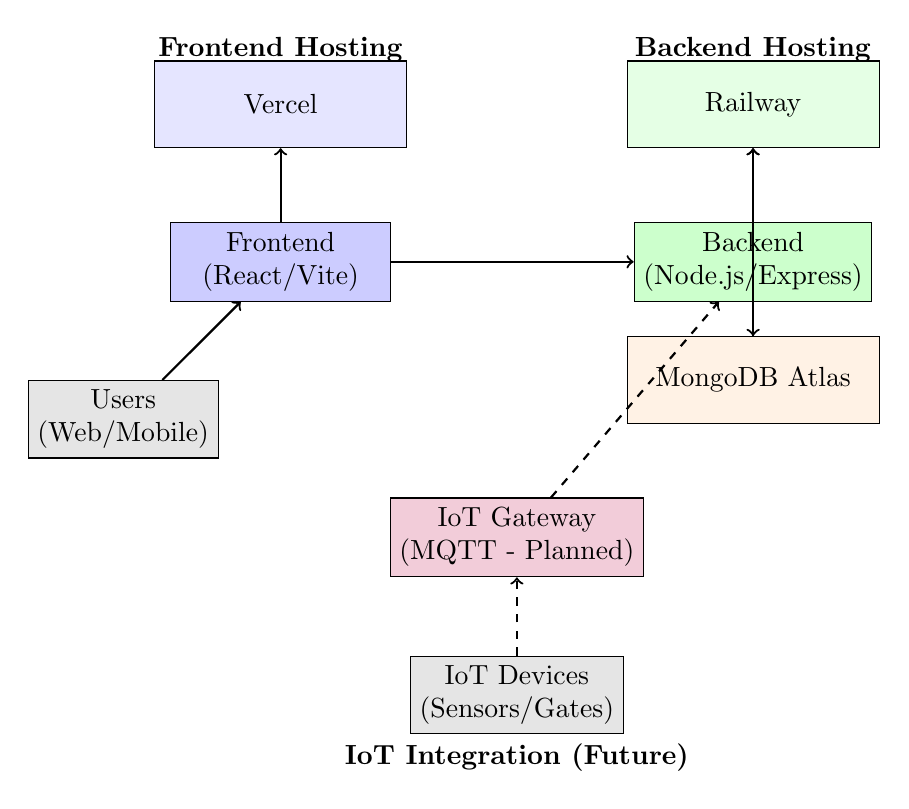
\begin{tikzpicture}[node distance=2.5cm, auto]
    % Cloud platforms - top tier
    \node[draw, fill=blue!10, minimum width=3.2cm, minimum height=1.1cm] (vercel) at (0,5) {Vercel};
    \node[draw, fill=green!10, minimum width=3.2cm, minimum height=1.1cm] (railway) at (6,5) {Railway};
    \node[draw, fill=orange!10, minimum width=3.2cm, minimum height=1.1cm] (mongodb) at (6,1.5) {MongoDB Atlas};

    % Application components - middle tier
    \node[draw, fill=blue!20, minimum width=2.8cm, minimum height=1cm, align=center] (frontend) at (0,3) {Frontend\\(React/Vite)};
    \node[draw, fill=green!20, minimum width=2.8cm, minimum height=1cm, align=center] (backend) at (6,3) {Backend\\(Node.js/Express)};
    \node[draw, fill=purple!20, minimum width=2.8cm, minimum height=1cm, align=center] (iot) at (3,-0.5) {IoT Gateway\\(MQTT - Planned)};

    % Users and devices - bottom tier
    \node[draw, fill=gray!20, minimum width=2.2cm, minimum height=0.8cm, align=center] (users) at (-2,1) {Users\\(Web/Mobile)};
    \node[draw, fill=gray!20, minimum width=2.4cm, minimum height=0.8cm, align=center] (devices) at (3,-2.5) {IoT Devices\\(Sensors/Gates)};

    % Connections
    \draw[->, thick] (users) -- (frontend);
    \draw[->, thick] (frontend) -- (backend);
    \draw[->, thick] (backend) -- (mongodb);
    \draw[->, thick, dashed] (devices) -- (iot);
    \draw[->, thick, dashed] (iot) -- (backend);

    % Platform connections
    \draw[->, thick] (frontend) -- (vercel);
    \draw[->, thick] (backend) -- (railway);
    \draw[->, thick] (mongodb) -- (railway);

    % Labels
    \node at (0,5.7) {\textbf{Frontend Hosting}};
    \node at (6,5.7) {\textbf{Backend Hosting}};
    \node at (3,-3.3) {\textbf{IoT Integration (Future)}};
\end{tikzpicture}
\caption{Deployment Architecture Overview}
\label{fig:deployment-arch}
\end{figure}

\subsection{Technology Stack}

\subsubsection{Frontend Technologies}

\paragraph{React 18 and Vite}
React 18 is used as the primary frontend library, allowing the team to break the UI into reusable, composable components. React supports a component-driven workflow, which improves collaboration, simplifies debugging, and helps the team implement complex features in smaller, maintainable pieces.

Vite serves as the frontend build tool and development server. It provides fast startup times and instant Hot Module Replacement (HMR), which keeps the development feedback loop short and reduces the time spent waiting for rebuilds.

\begin{figure}[H]
\centering

\includegraphics[width=0.8\linewidth]{react-vite.jpg}
\caption{React 18 and Vite frontend workflow}
\end{figure}

\paragraph{Tailwind CSS}
Tailwind CSS is the styling framework used for the frontend. Instead of writing raw CSS from scratch, the team uses Tailwind's utility classes to build responsive, modern layouts quickly. This approach reduces styling friction, improves visual consistency, and makes it easy to reuse patterns across components.

\paragraph{TypeScript}
TypeScript is used throughout the frontend to enforce type safety and provide better tooling support. Types help catch errors early, document data structures, and make the codebase easier to maintain as it evolves.

\subsubsection{Backend Technologies}

\paragraph{Node.js}
Node.js is the runtime for the backend, chosen for its event-driven, non-blocking I/O model. It allows the backend to handle many simultaneous requests efficiently and is a natural fit for JavaScript-based full-stack development.

\begin{figure}[H]
\centering

\includegraphics[width=0.35\linewidth]{Node.js_logo.svg.png}
\caption{Node.js runtime environment}
\end{figure}

\paragraph{Express}
Express is the server framework used to build RESTful API endpoints. It is lightweight and extensible, with a rich ecosystem of middleware and community packages. Express simplifies routing, request handling, and integration with authentication, validation, and logging.

\begin{figure}[H]
\centering

\includegraphics[width=0.7\linewidth]{express.png}
\caption{Express.js backend framework}
\end{figure}

\paragraph{MongoDB}
MongoDB is the NoSQL database used for application data storage. It stores data in a flexible JSON-like format, which aligns well with the application's domain models and simplifies schema evolution.

\begin{figure}[H]
\centering

\includegraphics[width=0.5\linewidth]{mongodb.png}
\caption{MongoDB document database}
\end{figure}

\paragraph{Mongoose}
Mongoose is used as an ODM to model MongoDB documents in the backend. It provides schema enforcement, validation, and convenient query APIs while preserving MongoDB's flexibility.

\subsubsection{Infrastructure and DevOps}

\paragraph{Docker Containerization}
The application is containerized with Docker. Docker allows the team to package the backend and frontend environments with all dependencies, ensuring consistent behavior across local development, staging, and production.

\begin{figure}[H]
\centering

\includegraphics[width=0.35\linewidth]{docker.png}
\caption{Docker containerization platform}
\end{figure}

\paragraph{Version Control and GitHub}
Source control is managed with Git and hosted on GitHub. GitHub provides a collaborative platform for branching, pull requests, and code review, while also integrating with automated workflows.

\paragraph{GitHub Actions CI/CD}
GitHub Actions is used for continuous integration and deployment. The repository is configured with workflows that automatically run linting, tests, and build steps on each push or pull request.

\begin{figure}[H]
\centering

\includegraphics[width=0.3\linewidth]{githubaction.png}
\caption{GitHub Actions CI/CD pipeline}
\end{figure}

\subsubsection{Supporting Technologies}

\paragraph{TypeScript (Backend)}
The backend also uses TypeScript to maintain consistency with the frontend and improve developer productivity. Shared type definitions across the stack reduce integration errors and improve code clarity.

\paragraph{JWT (JSON Web Tokens)}
JWT is used for stateless authentication. After successful sign-in, the system issues a token that the frontend includes in subsequent API calls, enabling secure access without server-side session state.

\paragraph{Pino}
Pino is the logging library used in the backend. It provides high-performance, structured logs that are easy to aggregate and analyze in production.

\paragraph{Jest and Vitest}
Jest is used for backend testing, and Vitest is used for frontend testing. Both frameworks support fast feedback, unit and integration testing, and code coverage reporting.

\paragraph{ESLint}
ESLint checks code quality and style on both frontend and backend code. It enforces consistent conventions, helps catch bugs early, and keeps the codebase maintainable.

\subsubsection{Moreover APIs}
Currently, several critical external integration points such as HCMUT\_SSO, HCMUT\_DATACORE, BKPAY, and the IoT Device APIs are implemented as mock services to facilitate the current phase of development and testing. Upon final deployment, the IoT Devices are planned to be managed and orchestrated through the MQTT protocol to ensure high-performance, real-time communication across the campus infrastructure.

\subsection{Business Flow Integration}

\subsubsection{Authentication Flow}
\begin{enumerate}
\item User accesses frontend application on Vercel
\item Frontend redirects to HCMUT SSO for authentication
\item SSO returns JWT token to frontend
\item Frontend stores token and calls backend APIs
\item Backend validates JWT with Railway-hosted service
\end{enumerate}

\subsubsection{Billing and Payment Flow}
\begin{enumerate}
\item User initiates parking session via frontend
\item Backend calculates fees using pricing policies
\item Payment request sent to BKPay integration
\item Payment confirmation updates session status in MongoDB
\item Real-time updates sent to frontend via WebSocket/SSE
\end{enumerate}

\subsubsection{IoT Data Flow (Planned)}
\begin{enumerate}
\item IoT sensors publish data to MQTT topics
\item MQTT gateway receives and processes messages
\item Processed data sent to Railway backend
\item Backend updates parking slot status in MongoDB
\item Real-time updates broadcast to connected frontends
\end{enumerate}

\subsection{Security Considerations}

\subsubsection{Data Protection}
\begin{itemize}
\item HTTPS encryption for all communications
\item JWT tokens for API authentication
\item MongoDB access control and encryption
\item Secure environment variable management
\end{itemize}

\subsubsection{Network Security}
\begin{itemize}
\item Vercel automatic HTTPS certificates
\item Railway firewall and access controls
\item API rate limiting and request validation
\item CORS configuration for frontend-backend communication
\end{itemize}

\subsection{Scalability and Performance}

\subsubsection{Frontend Scaling}
\begin{itemize}
\item Vercel's global CDN for low-latency content delivery
\item Static asset optimization and caching
\item Automatic scaling based on traffic
\end{itemize}

\subsubsection{Backend Scaling}
\begin{itemize}
\item Railway's horizontal scaling capabilities
\item MongoDB connection pooling and indexing
\item API response caching and optimization
\end{itemize}

\subsubsection{Database Scaling}
\begin{itemize}
\item MongoDB Atlas auto-scaling
\item Read/write splitting capabilities
\item Backup and disaster recovery
\end{itemize}